\documentclass[reqno,12pt]{article}

\usepackage{setspace,graphicx,epstopdf,amsmath,amsfonts,amssymb,amsthm}
\usepackage{datetime,enumitem,subfigure,rotating,fancyvrb}
\usepackage{listings}
\usdate

\begin{document}

\title{\textbf{CS 598 Homework 1}}
  
\author{Mohan Sun\footnote{Even if this document use "we" and "our", the homework is done
by only Mohan "Fred" Sun without any collaboration. Netid: mohans2}}

\date{\vspace{-5ex}}

\maketitle

\doublespacing

\noindent We implement a fully connected one-hidden-layer neural network and train the model
with MNIST data. Figure \ref{fig:res} shows training results and timing. Our model have 
an accuracy of 97.97\% which satisfies the requirement of the assignment.

\textit{Model} the model is a modified and extended version of Logisticregression.py. We keep the 
i/o and data processing part, keep the structure of Epoch loop, mini-batch loop, and forward as well as 
backward as function. We modified forward to: 

\begin{lstlisting}
def forward(x,y, model):
    Z = model['W'] @ x + model['b1']
    H = sigmoid(Z)
    U = model['C'] @ H + model['b2']
    p = softmax_function(U)
    return Z, H, p
\end{lstlisting}

\newpage
and backward to:

\begin{lstlisting}
def backward(x, y, Z, H, p, model, model_grads):
    dU = np.copy(p)
    dU[y] = dU[y] - 1
    dC = dU @ H.T
    delta = model['C'].T @ dU
    db1 = delta * sigmoidp(Z)
    dW = db1 @ x.T
    model_grads['W']=dW
    model_grads['b1']=db1
    model_grads['b2']=dU
    model_grads['C']=dC
    return model_grads
\end{lstlisting}

This basically reflects the model used in lecture notes. The only difference here is that we use sigmoid
instead of ReLU to avoid overflow issue with exponentials in softmax.

\textit{parameters} For this model, we set $D_h = 100$ and $LR^{(0)}=0.1$. $LR$ is scaled down by $10$
for every $5$ epochs.

\begin{figure}[!t]
  \centering 
  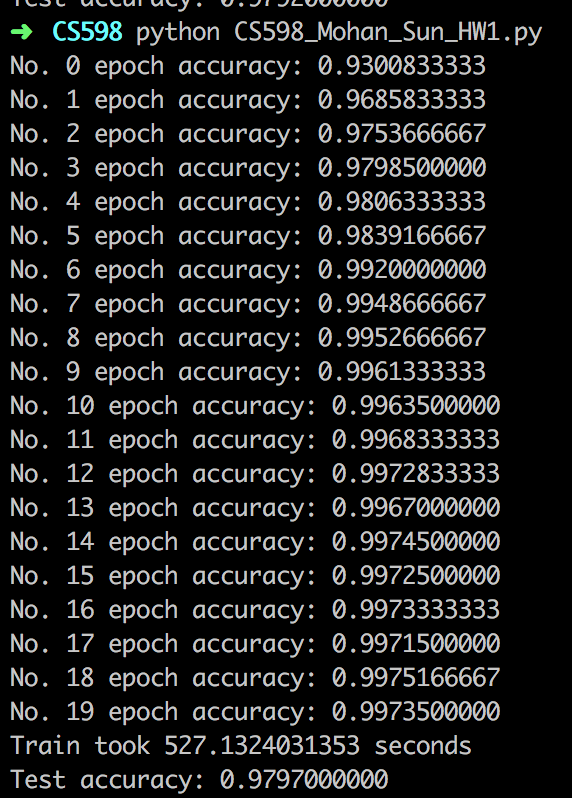
\includegraphics[width = \textwidth]{HW1_result.png}

  \vskip0.25cm

  \caption{\textnormal{\bf Neural Network Training Result and Timing.} Our model have a 
  test accuracy of 97.97\% in the last run. Training takes approximately 527 seconds.}
  \label{fig:res}
\end{figure}

\end{document}
